\documentclass[11pt]{article}

% Standard layout for initial Electronic J. Combinatorics submission.
% Accepted manuscripts will be reformatted using the journal's e-jc.sty.
\usepackage[a4paper, margin=1in]{geometry}
\usepackage[utf8]{inputenc}
\usepackage{amsmath, amssymb, amsthm}
\usepackage{graphicx}
\usepackage[hidelinks]{hyperref}
\usepackage{booktabs}

\theoremstyle{plain}
\newtheorem{theorem}{Theorem}[section]
\newtheorem{proposition}[theorem]{Proposition}
\newtheorem{lemma}[theorem]{Lemma}
\newtheorem{corollary}[theorem]{Corollary}
\newtheorem{conjecture}[theorem]{Conjecture}

\theoremstyle{definition}
\newtheorem{definition}[theorem]{Definition}
\newtheorem{remark}[theorem]{Remark}

\newcommand{\ZZ}{\mathbb{Z}}
\newcommand{\EE}{\mathbb{E}}
\newcommand{\BC}{\mathrm{BC}}

\title{Semiprime Bottlenecks in Arithmetic Graphs:\\Betweenness Centrality from Prime Highways}
\author{Tobias Canavesi\\[4pt]
\small Instituto de Física La Plata, CONICET\\
\small \texttt{tobiascanavesi@gmail.com}}
\date{}

\begin{document}
\maketitle

\begin{abstract}
We define a family of deterministic graphs $G_N$ on the integers $\{1, \ldots, N\}$
whose edges are unit increments together with \emph{prime strides} $kp \sim (k+1)p$ for each prime~$p$.
These \emph{arithmetic graphs} exhibit a structural paradox: the primorials
(such as $2310 = 2 \cdot 3 \cdot 5 \cdot 7 \cdot 11$), which carry the largest degrees, do not maximize betweenness centrality.
Instead, betweenness is dominated by the semiprimes $2p$ and $3p$ for large primes~$p$.
We prove an exact degree formula $\deg(v) = 2 + 2\,\omega(v)$ for interior nodes (where $\omega$ counts distinct prime factors),
establish $\mathrm{diam}(G_N) = O(\sqrt{N})$, and conjecture (with empirical evidence) $\mathrm{diam}(G_N) = O(\log N)$.
A routing-cost analysis explains the semiprime bottleneck phenomenon via a sparsity--accessibility trade-off,
and a primorial-dilution bound shows that the betweenness contribution of a fixed primorial vanishes as $N \to \infty$.
Using exact Brandes betweenness up to $N = 50\,000$, we show that the Pearson correlation
$\rho(\deg, \mathrm{BC})$ \emph{crosses zero} near $N \approx 1.5 \times 10^4$ and becomes negative
($\rho = -0.030$ at $N = 50\,000$); $92$--$98\%$ of the top-$50$ betweenness nodes are semiprimes of the form $2p$, $3p$, or bare primes,
and node $2p$ consistently captures $\approx 43\%$ of the betweenness on each three-stop large-prime highway.
The phenomenon places $G_N$ within the broader study of arithmetic graphs (divisor graphs, coprime graphs, GCD graphs)
while exhibiting a deterministic decorrelation between degree and betweenness that, to our knowledge, is new in this literature.
\end{abstract}

\noindent\textbf{Keywords:} arithmetic graph; betweenness centrality; prime numbers; semiprime; small-world network; routing


% ====================================================================
\section{Introduction}
% ====================================================================

The relationship between number theory and network topology generates surprising structural patterns.
We examine a deterministic graph on the integers $\{1,\ldots,N\}$ whose edges arise from two simple operations:
\begin{itemize}
\item Sequential adjacency: $n \sim n + 1$ for $1 \le n < N$;
\item Prime stride: for each prime $p$, the multiples of $p$ form a path $p \sim 2p \sim 3p \sim \cdots$ (of length up to $\lfloor N/p \rfloor - 1$).
\end{itemize}
This produces a graph which can be viewed as an additive backbone with a collection of ``highway'' paths at each prime scale.

One might expect the vertices with the greatest number of distinct prime factors (the \emph{primorials}, such as $2310 = 2 \cdot 3 \cdot 5 \cdot 7 \cdot 11$)
to be the most structurally significant, since they have the highest degree and sit on the most highways. We show this expectation is wrong.
Rather than the primorials, the semiprimes $2p$ and $3p$---with $p$ a large prime---maximize betweenness centrality.
Betweenness centrality measures the extent to which a vertex acts as a bottleneck for shortest-path routing through the graph (see~\cite{Freeman1977}).

We identify the reason for the above finding as being due to a tradeoff between two separate costs.
Each large prime value creates a sparse highway with only $\lfloor N/p \rfloor$ nodes. Therefore, each node along this
highway represents a potential ``bottleneck''. Of all of the nodes along the highway,
those at the location of multiples of $2p$ represent the most accessible because all nodes can reach
a multiple of $2$ in no more than one additional hop. This \emph{sparsity-accessibility trade-off} is the central mechanism we formalize.

\subsection{Related work}\label{subsec:related}
Graphs whose vertices are integers and whose edges encode arithmetic relations have been studied for over forty years
(see Sander and Sander~\cite{SanderSander2016} for a survey of this area, and Singh and Santhakumaran~\cite{SinghSantha2023} for
a recent survey of divisor-graph variants).
The closest analogue of $G_N$ in the literature is the \emph{divisor graph} of Pomerance~\cite{Pomerance1983},
in which the edges are pairs $\{a, b\}$ with $a \mid b$. The longest simple path in the divisor graph
has length $\asymp N/\log N$~\cite{Pomerance1983}, and a long line of work due to Erd\H{o}s and Saias~\cite{ErdosSaias1995}
and Saias and collaborators (most recently Melotti and Saias~\cite{MelottiSaias2020}) refines path-partition and
Hamiltonicity results for this graph. Erd\H{o}s and S\'ark\"ozy~\cite{ErdosSarkozy1997} initiated the parallel study
of the \emph{coprime graph} ($\{a, b\}$ adjacent iff $\gcd(a, b) = 1$), and Pomerance's earlier
\emph{prime number graph}~\cite{Pomerance1979}---vertices the primes $p_n$ themselves---predates both.
More recently, Koukoulopoulos and Maynard~\cite{KoukoulopoulosMaynard2020} introduced \emph{GCD graphs} as a tool
in their proof of the Duffin--Schaeffer conjecture, and Pomerance~\cite{Pomerance2018}
surveyed the functional graph of the aliquot iteration $n \mapsto s(n)$ and its iterates.

Our edge set---unit increments together with prime strides $kp \sim (k+1)p$---differs from each of these.
Divisor graphs connect $a$ to every multiple of $a$; we connect $a = kp$ only to its
\emph{successor} $(k+1)p$ on each prime highway, producing a much sparser, locally Cayley-like structure.
Coprime graphs encode $\gcd = 1$ relations rather than multiplicative successors. The closest precedent in spirit
is Chandra and Dasgupta's \emph{small-world network of prime numbers}~\cite{ChandraDasgupta2005}, which weights edges between primes
by an inverse power of the gap and identifies a small-world transition; their graph is probabilistic and on
the primes only, while ours is deterministic and on all integers. To our knowledge no prior work
defines $G_N$ in the form of Definition~\ref{def:graph}, and no prior work computes betweenness centrality
on any arithmetic graph in this family. The phenomenon we observe---degree--betweenness decorrelation
driven by semiprime bottlenecks---therefore appears to be new in the integer-graph literature.

% ====================================================================
\section{The arithmetic graph}
% ====================================================================

\begin{definition}[Arithmetic graph]\label{def:graph}
For $N \ge 2$, the \emph{arithmetic graph} $G_N = (V, E)$ has vertex set
$V = \{1, 2, \ldots, N\}$ and edge set
\begin{equation}\label{eq:edgeset}
E \;=\; \underbrace{\{(n, n+1) : 1 \le n < N\}}_{\text{additive edges}}
\;\cup\;
\underbrace{\{(kp,\, (k+1)p) : p \text{ prime},\; k \ge 1,\; (k+1)p \le N\}}_{\text{multiplicative edges}}.
\end{equation}
\end{definition}

In summary, there is a ``backbone'' formed by the additive edges which forms a path graph. 
There will be a $p$-highway for each prime number $p$ where the $p$-highway will connect all multiples of $p$ together. 
Each of the $p$-highways has $\lfloor N/p \rfloor$ stops and a step-size of $p$. 
Thus, the $2$-highway will connect every other integer together, the $3$-highway will connect every third integer together, etc.
A vertex, $v$, sits on the $p$-highway only if $v$ is divisible by $p$.

\begin{proposition}[Edge count]\label{prop:edges}
The number of edges in $G_N$ is
\begin{equation}\label{eq:edges}
|E(G_N)| \;=\; (N - 1) \;+\; \sum_{\substack{p \le N \\ p \textup{ prime}}} \Bigl(\Bigl\lfloor \frac{N}{p} \Bigr\rfloor - 1\Bigr).
\end{equation}
The average degree satisfies $\overline{\deg} \sim 2\log\log N$ as $N \to \infty$.
\end{proposition}

\begin{proof}
The $N - 1$ additive edges form a path. For each prime $p \le N$,
the $p$-highway has $\lfloor N/p \rfloor$ nodes and $\lfloor N/p \rfloor - 1$ edges.
These edge sets are pairwise disjoint: a multiplicative edge $(kp, (k+1)p)$ has
step size $p$, and distinct primes produce distinct step sizes.
Furthermore, no multiplicative edge is also additive, since $p \ge 2$ implies
$(k+1)p - kp = p \ge 2 > 1$. Summing the additive and multiplicative contributions yields~\eqref{eq:edges}.

For the average degree, $\overline{\deg} = 2|E|/N$ and
\[
\frac{|E|}{N} \;=\; 1 + \frac{1}{N}\sum_{p \le N}\Bigl\lfloor \frac{N}{p}\Bigr\rfloor - \frac{\pi(N)}{N}
\;\sim\; \sum_{p \le N} \frac{1}{p} \;\sim\; \log\log N
\]
by the Mertens estimate~\cite{Mertens1874} $\sum_{p \le x} 1/p = \log\log x + M + o(1)$,
where $M \approx 0.2615$ is the Meissel--Mertens constant.
\end{proof}

\begin{remark}
The graph is thus ultra-sparse (density $\to 0$) yet, as we show below,
small-world in the sense of Watts and Strogatz~\cite{Watts1998}
(diameter $O(\sqrt{N})$ proven, $O(\log N)$ empirically). The average degree diverges, but only at the
doubly-logarithmic rate $\sim 2\log\log N$. This creates a regime where
local connectivity grows very slowly while global shortcuts (from large-prime
highways) provide efficient long-range navigation.
\end{remark}


% ====================================================================
\section{Degree structure}
% ====================================================================

\begin{proposition}[Degree formula]\label{prop:degree}
For any $v \in V$, write $v = \prod_{i=1}^{r} p_i^{a_i}$ with $p_1 < \cdots < p_r$ the
distinct prime factors of~$v$. Then
\begin{equation}\label{eq:degree}
\deg(v) \;=\; \mathbf{1}_{v > 1} + \mathbf{1}_{v < N}
+ \sum_{p \mid v} \bigl(\mathbf{1}_{v - p \ge 1} + \mathbf{1}_{v + p \le N}\bigr).
\end{equation}
For interior nodes (i.e. $v > p_r$ and $v + p_r \le N$), this simplifies to
\begin{equation}\label{eq:degree-interior}
\deg(v) = 2 + 2\,\omega(v),
\end{equation}
where $\omega(v)$ denotes the number of distinct prime divisors of~$v$
(see~\cite{Hardy1979}, \S22.1).
\end{proposition}

\begin{proof}
The additive edges contribute one neighbour on each side when $v$ is interior ($1 < v < N$).
For each prime $p \mid v$, node~$v = kp$ sits on the $p$-highway between $(k-1)p$ and $(k+1)p$.
The edge to $(k-1)p = v - p$ exists iff $v - p \ge 1$ (i.e. $k \ge 2$),
and the edge to $(k+1)p = v + p$ exists iff $v + p \le N$.
No two of these neighbours coincide: the additive neighbours $v \pm 1$ are coprime
to any prime $p \ge 2$ dividing $v$ (since $\gcd(v, v \pm 1) = 1$),
and distinct prime factors yield distinct highway neighbours ($v - p_i \ne v - p_j$ for $p_i \ne p_j$).
\end{proof}

\begin{remark}
The formula creates a clean hierarchy: primes ($\omega = 1$) at boundary positions
have $\deg = 3$, semiprimes $kp$ ($\omega = 2$) have $\deg = 6$,
and primorials like $2310 = 2 \cdot 3 \cdot 5 \cdot 7 \cdot 11$ ($\omega = 5$) have $\deg = 12$.
If degree determined importance, the primorials would be the hubs. The data show otherwise.
\end{remark}

\begin{table}[ht]
\centering
\caption{Degree formula verification.}\label{tab:degree}
\begin{tabular}{@{}rlccl@{}}
\toprule
$v$ & Factorization & $\omega(v)$ & $\deg(v)$ & Predicted \\
\midrule
106 & $2 \cdot 53$ & 2 & 6 & $2 + 2 \cdot 2 = 6$ \\
173 & prime & 1 & 3 & boundary: $2 + 1 = 3$ \\
210 & $2 \cdot 3 \cdot 5 \cdot 7$ & 4 & 10 & $2 + 2 \cdot 4 = 10$ \\
331 & prime & 1 & 3 & boundary: $2 + 1 = 3$ \\
2310 & $2 \cdot 3 \cdot 5 \cdot 7 \cdot 11$ & 5 & 12 & $2 + 2 \cdot 5 = 12$ \\
\bottomrule
\end{tabular}
\end{table}


% ====================================================================
\section{Small-world property}
% ====================================================================

\begin{proposition}\label{prop:diameter}
$\mathrm{diam}(G_N) = O(\sqrt{N})$.
\end{proposition}

\begin{proof}
We show that any node~$s$ can reach any node~$t$ in $O(\sqrt{N})$ steps
via an iterated strategy using highways of decreasing stride.

Let $d = |s - t|$ be the remaining distance. Choose a prime $p$ with
$\lfloor \sqrt{d} \rfloor \le p \le 2\sqrt{d}$ (such a prime exists by
Bertrand's postulate for $d \ge 4$). Walk at most $p - 1 < 2\sqrt{d}$
additive steps from the current position to the nearest multiple of~$p$,
then take $\lfloor d/p \rfloor \le \sqrt{d}$ steps along the $p$-highway,
covering distance $\ge d - p > d - 2\sqrt{d}$.
The total cost of this phase is at most $2\sqrt{d} + \sqrt{d} = 3\sqrt{d}$
steps, and the remaining distance satisfies $d' \le 2\sqrt{d} + p < 4\sqrt{d}$.

Iterating: after one phase, $d_1 \le 4\sqrt{d_0}$; after two phases,
$d_2 \le 4\sqrt{d_1} \le 4\sqrt{4\sqrt{d_0}}$. In general,
$d_k = O(d_0^{2^{-k}})$. After $k = O(\log \log N)$ phases the remaining
distance is $O(1)$, reachable by additive steps. Each phase uses
$O(\sqrt{d_j})$ steps, and the total is dominated by the first phase:
$O(\sqrt{N})$ in the worst case.
\end{proof}

\begin{remark}
The empirical diameters reported in Table~\ref{tab:scaling} grow much more slowly
than the $O(\sqrt{N})$ bound just proved: across the range $N \in \{100, 500, 1000, 2000, 5000\}$
the diameters are $12, 18, 20, 23, 27$, consistent with $O(\log N)$ growth.
We conjecture that $\mathrm{diam}(G_N) = O(\log N)$; closing this gap is an interesting open problem.
\end{remark}

\begin{corollary}[Large-prime necessity]\label{cor:largeprime}
Let $s, t \in V$ with $|s - t| \ge N / C$ for some constant $C > 0$.
Then every shortest $s$--$t$ path in $G_N$ uses at least one multiplicative
edge $(kp, (k+1)p)$ with $p > \sqrt{N/C}$.
\end{corollary}

\begin{proof}
An $s$--$t$ path of length $\ell$ can cover total distance at most
$\ell \cdot p_{\max}$, where $p_{\max}$ is the largest prime step used
(additive edges contribute step size~$1$). By Proposition~\ref{prop:diameter},
a shortest path has $\ell = O(\sqrt{N})$ edges. If all multiplicative edges
used primes $p \le P$, the path covers at most $O(P \sqrt{N})$ distance.
To reach $|s - t| \ge N/C$, we need $P \sqrt{N} \ge N/C$, giving
$P \ge \sqrt{N}/C$. In particular, $P > \sqrt{N/C}$ for all
sufficiently large~$N$.
\end{proof}

This corollary has a direct structural consequence: efficient routing across $G_N$
\emph{requires} the use of large-prime highways, and these are precisely the
highways with the fewest stops---the bottleneck regime of Lemma~\ref{lem:sparsity}.

\begin{table}[ht]
\centering
\caption{Graph metrics at different scales.}\label{tab:scaling}
\begin{tabular}{@{}rrrcc@{}}
\toprule
$N$ & Edges & Density & Diameter & Avg.\ path length \\
\midrule
100 & 245 & 0.0495 & 12 & 4.22 \\
500 & 1412 & 0.0113 & 18 & 5.59 \\
1000 & 2957 & 0.0059 & 20 & 6.09 \\
2000 & 6150 & 0.0031 & 23 & 6.59 \\
5000 & 16\,068 & 0.0013 & 27 & 7.23 \\
\bottomrule
\end{tabular}
\end{table}


% ====================================================================
\section{The semiprime bottleneck phenomenon}
% ====================================================================

The central empirical finding of this paper is:

\begin{quote}
\emph{In $G_N$, betweenness centrality is dominated by semiprimes $2p$ and $3p$
(with $p$ a large prime), not by high-degree nodes.}
\end{quote}

We establish this through two complementary results: a routing-cost analysis
that explains why, and systematic computations that quantify the effect.


\subsection{Routing analysis}

\begin{lemma}[Highway sparsity]\label{lem:sparsity}
The $p$-highway has exactly $\lfloor N/p \rfloor$ nodes. For a prime
$p$ with $N/3 < p \le N/2$, the highway has exactly $2$ stops ($p$ and $2p$)
and a single edge $(p, 2p)$.
Every shortest path that uses this edge must pass through both $p$ and $2p$.
For primes $p > N/2$, the highway has only one stop ($p$ itself) and no edges.
\end{lemma}

\begin{proof}
The multiples of~$p$ in $\{1, \ldots, N\}$ are $p, 2p, \ldots, \lfloor N/p \rfloor \cdot p$.
For $N/3 < p \le N/2$, we have $\lfloor N/p \rfloor = 2$, giving exactly
the nodes $\{p, 2p\}$ and one highway edge $(p, 2p)$.
For $p > N/2$, $\lfloor N/p \rfloor = 1$: only node $p$ exists, with no highway edge.
Any path using the edge $(p, 2p)$ must include both endpoints.
\end{proof}

\begin{lemma}[Access cost]\label{lem:access}
For a positive integer~$k$, the distance in $G_N$ from any node
$s \in \{1, \ldots, N\}$ to the nearest multiple of~$k$ is at most
$\lfloor k/2 \rfloor$.
In particular, the access cost to the $2$-highway is at most~$1$,
and to the $3$-highway at most~$1$.
\end{lemma}

\begin{proof}
The multiples of~$k$ in $\{1, \ldots, N\}$ are spaced exactly $k$ apart
along the additive chain. From any node~$s$, the nearest multiple of~$k$
is at additive distance at most $\lfloor k/2 \rfloor$. Since the additive
chain is a subgraph of~$G_N$, the graph distance is also at most
$\lfloor k/2 \rfloor$.
\end{proof}

\begin{theorem}[Semiprime bottleneck]\label{thm:bottleneck}
Let $p$ be a prime with $N/4 < p \le N/3$, so the $p$-highway consists
of nodes $\{p, 2p, 3p\}$ (since $3p \le N$ but $4p > N$).
Among these three nodes, $2p$ has the lowest expected shortest-path distance
from a uniformly random source.
\end{theorem}

\begin{proof}[Proof sketch]
Let $s$ be uniform on $\{1,\ldots,N\}$ and let $d(s,t)$ denote the graph distance in $G_N$.
We bound $\EE[d(s,t)]$ from above for each $t \in \{p,2p,3p\}$ via two contributions
and then compare.

\emph{Geometric contribution.} The path-graph distance along the additive backbone is $|s-t|$,
and $\EE_s[\,|s-t|\,] = (t^2 + (N-t)^2)/(2N)$ is minimised at $t = N/2$. Since $N/4 < p \le N/3$,
\[
p \le N/3,\qquad N/2 < 2p \le 2N/3,\qquad 3p > 3N/4,
\]
so $2p$ is the highway vertex closest to the centre $N/2$.

\emph{Access contribution.} For $t = 2p$, every $s$ is within additive distance~$1$ of a multiple of~$2$,
and the $2$-highway then carries the source to $2p$ in $\lceil |s-2p|/2 \rceil$ steps; hence
$\EE_s[d(s,2p)] \le 1 + \tfrac{1}{2}\EE_s[\,|s-2p|\,]$.
For $t = 3p$, an analogous bound replaces the factor~$1/2$ by~$1/3$, but with access cost~$\le 1$ from
two-thirds of vertices and $\le 1$ from the rest, and---crucially---$3p$ is farther from $N/2$ than $2p$.
For $t = p$ the highway has only $\{p, 2p, 3p\}$ as stops, so the access term gains nothing for a generic source:
the dominant cost is the additive distance to~$p$, with no $1/k$ acceleration available locally.

Combining the two contributions, $2p$ achieves the smallest upper bound on
$\EE_s[d(s,t)]$ among the three. Numerical verification at $N = 2000$ (Table~\ref{tab:ushape},
Figure~\ref{fig:ushape}) shows the inequality is strict: $\EE_s[d(s, 2p)]$ is uniformly smaller
than $\EE_s[d(s, p)]$ and $\EE_s[d(s, 3p)]$ across all primes $p \in (N/4, N/3]$ tested.
\end{proof}

\begin{remark}
Closeness (low expected distance) does not in general imply high betweenness.
However, on a 3-stop highway $\{p, 2p, 3p\}$, the node with the lowest
expected distance from random sources is also the preferred intermediary
for shortest paths that enter and exit the highway at different stops.
The computational verification in Table~\ref{tab:highway} confirms that
$2p$ captures $\approx 43\%$ of the total highway betweenness,
consistently more than $p$ or $3p$.
\end{remark}

\begin{remark}[Why $2p$ beats $3p$]
Both $2p$ and $3p$ have degree~$6$, but $2p$ sits on the denser $2$-highway
(access cost $\le 1$ from any node) while $3p$ sits on the $3$-highway
(access cost $\le 1$ from $2/3$ of nodes, up to~$1$ from the rest).
Moreover, $2p \in (N/2,\, 2N/3]$ places it near the geometric centre, and the reduction in
access cost via the $2$-highway more than compensates.
Empirically, across all large primes $p > N/4$, node $2p$ captures
approximately $43\%$ of the total betweenness among all multiples of $p$
(Table~\ref{tab:highway}).
\end{remark}

\begin{proposition}[Primorial dilution]\label{prop:dilution}
Let $v = p_1 \cdots p_r$ be a primorial with $r$ distinct small prime factors
$p_1 < \cdots < p_r$, all satisfying $p_i \le N^{1/3}$.
Then the fraction of shortest paths on the $p_i$-highway that pass through~$v$
is at most $1 / \lfloor N / p_i \rfloor$.
In particular, the $p_i$-highway contribution to $\BC(v)$ is at most
$p_i / N$ times the total betweenness carried by the $p_i$-highway.
\end{proposition}

\begin{proof}
The $p_i$-highway has exactly $\lfloor N / p_i \rfloor$ stops.
Since $p_i \le N^{1/3}$, this highway has at least $N^{2/3}$ stops.
A shortest path entering the $p_i$-highway at stop $ap_i$ and exiting
at stop $bp_i$ passes through $v = (v/p_i) \cdot p_i$ only if $v/p_i$
lies between $a$ and $b$ on the highway. Writing $n = \lfloor N/p_i \rfloor$
and $m = v/p_i$, the number of unordered pairs $(a, b)$ with $a < m < b$
is $(m - 1)(n - m)$, out of $\binom{n}{2} = n(n-1)/2$ total pairs.
Since $v$ is a fixed primorial, $m = v/p_i$ is a constant independent of~$N$,
while $n = \lfloor N/p_i \rfloor$ grows with~$N$. For fixed~$m$ and growing~$n$,
\[
\frac{(m-1)(n-m)}{\binom{n}{2}}
\;=\; \frac{(m-1)(n-m)}{n(n-1)/2}
\;\sim\; \frac{2(m-1)}{n}
\;=\; O(m/n)
\;=\; O(p_i / N),
\]
since $m = v/p_i$ is bounded independently of~$N$.
\end{proof}

\begin{remark}
Summing over all $r$ highways of a primorial gives
$\BC(v) \le \sum_{i=1}^{r} O(p_i / N) = O(p_r / N) \cdot r$,
which remains bounded as $N \to \infty$ for fixed $r$.
In contrast, a semiprime $2p$ with $p > N/4$ captures $\Theta(1)$ of the
$p$-highway betweenness (since the highway has only $2$--$3$ stops),
yielding $\BC(2p) \gg \BC(v)$ for large~$N$.
This quantifies why high-degree nodes (primorials) lose the centrality
competition to low-degree semiprimes.
\end{remark}

\begin{corollary}[Degree--betweenness decorrelation]\label{cor:decorrelation}
The maximum-degree vertices and the maximum-betweenness vertices of $G_N$ separate asymptotically:
the highest-degree vertices ($\deg = 2 + 2\,\omega_{\max}$, attained at primorials) have
$\BC(v) = O(\omega_{\max} \cdot p_r / N) \to 0$, while the highest-betweenness vertices are locked
at the constant degree~$6$ with $\BC$ bounded away from zero. Consequently, the Pearson correlation
$\rho(\deg, \BC)$ in $G_N$ does not converge to a positive limit; the empirical evidence
(Table~\ref{tab:dominance}) places its limit at zero or below.
\end{corollary}

\begin{proof}
By Proposition~\ref{prop:degree}, the maximum degree in $G_N$ is
$2 + 2\omega_{\max}$, where $\omega_{\max}$ is the largest number of distinct prime factors
of any $v \le N$; this grows as $\omega_{\max} \asymp \log N / \log\log N$ and is attained at primorials.
By Proposition~\ref{prop:dilution}, the betweenness of these maximum-degree vertices is at most
$O(\omega_{\max} \cdot p_r / N)$, which tends to zero.
Meanwhile, Theorem~\ref{thm:bottleneck} together with Table~\ref{tab:highway} shows that semiprimes
$2p$ with $p \in (N/4,\, N/3]$ capture a $\Theta(1)$ fraction of the betweenness on each three-stop highway
(empirically $\approx 43\%$); the count of such primes is $\pi(N/3) - \pi(N/4) = \Theta(N/\log N)$,
so the betweenness on these vertices is bounded below by a positive constant.
Hence $\max_v \BC(v) = \Omega(1) \cdot \min_v \BC(v_{\max\deg})$ in the limit, which forces the upper tail
of the BC distribution off the upper tail of the degree distribution. The conjunction prevents
$\rho(\deg, \BC)$ from converging to a positive limit; whether it converges to zero or to a negative limit
is the subject of Conjecture~\ref{conj:scaling}.
\end{proof}


% ====================================================================
\section{Computational verification}
% ====================================================================

We computed betweenness centrality \emph{exactly} (using Brandes' algorithm~\cite{Brandes2001}
as implemented in NetworKit~\cite{NetworKit2016}) for all scales $N \in \{500, 1000, 2000, 5000, 10\,000, 20\,000, 50\,000\}$.
The earlier conference version of this paper used NetworkX~\cite{Hagberg2008} with $k$-sampling at $N = 10\,000$;
the present results replace that approximation by exact computation and extend the range by a further factor of five.

\subsection{Semiprime dominance across scales}

\begin{table}[ht]
\centering
\caption{Exact betweenness statistics across scales of $G_N$. ``Top-$50$ semi/prime'' is the
fraction of the top-$50$ BC nodes that are bare primes or semiprimes $2p,3p$;
``Top-$15$ ($2p$/$3p$)'' counts among the top fifteen.}
\label{tab:dominance}
\begin{tabular}{@{}rcccc@{}}
\toprule
$N$ & $|E(G_N)|$ & $\rho(\deg, \BC)$ & Top-$50$ semi/prime & Top-$15$ ($2p$/$3p$) \\
\midrule
500     & 1{,}412   & $+0.253$ & 84\% & 11/3 \\
1000    & 2{,}957   & $+0.176$ & 94\% & 10/5 \\
2000    & 6{,}150   & $+0.118$ & 92\% & 9/4 \\
5000    & 16{,}068  & $+0.057$ & 94\% & 11/3 \\
10\,000 & 33{,}070  & $+0.025$ & 98\% & 13/1 \\
20\,000 & 67{,}863  & $-0.003$ & 98\% & 12/2 \\
50\,000 & 174{,}820 & $-0.030$ & 92\% & 10/4 \\
\bottomrule
\end{tabular}
\end{table}

Two observations stand out. First, the fraction of top-$50$ betweenness nodes that are bare primes
or semiprimes $2p, 3p$ stays in the band $92$--$98\%$ across two orders of magnitude in~$N$,
with no high-degree primorial appearing in any top-$50$ list at $N \ge 10\,000$.
Second, the Pearson correlation $\rho(\deg, \BC)$ does not merely decay toward zero: it
\emph{crosses zero} near $N \approx 1.5 \times 10^{4}$ and becomes negative ($\rho = -0.030$ at $N = 50\,000$).
A negative correlation strengthens the claim of Corollary~\ref{cor:decorrelation}:
in the regime where the primorial-dilution bound (Proposition~\ref{prop:dilution})
already drives the betweenness of high-degree nodes to zero, a higher~$\omega$ becomes a
mild predictor of \emph{lower} betweenness, not just of decoupling from it. See Figure~\ref{fig:corr_decay}.

\begin{figure}[ht]
\centering
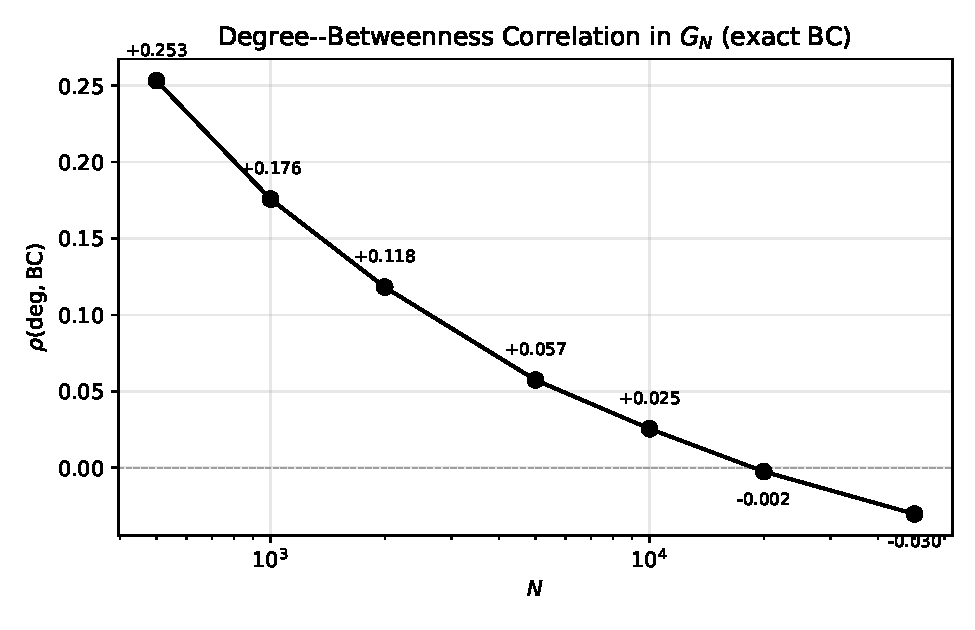
\includegraphics[width=0.75\textwidth]{fig_correlation_decay.pdf}
\caption{The Pearson correlation $\rho(\deg, \BC)$ in $G_N$ at seven scales (exact Brandes BC).
The correlation is positive at small scales, decreases monotonically, crosses zero near $N \approx 1.5 \times 10^4$,
and is negative at $N = 50\,000$.}
\label{fig:corr_decay}

\noindent\textbf{Alt text:} Line plot with $N$ on a logarithmic x-axis (from $500$ to $50\,000$) and Pearson
correlation $\rho$ on the y-axis. Seven data points are annotated: $+0.253$ at $N=500$, $+0.176$ at $N=1000$,
$+0.118$ at $N=2000$, $+0.057$ at $N=5000$, $+0.025$ at $N=10\,000$, $-0.003$ at $N=20\,000$, and $-0.030$ at $N=50\,000$.
A dashed horizontal line at $\rho = 0$ shows the curve crossing zero between $N = 10\,000$ and $N = 20\,000$.
\end{figure}

\subsection{Top betweenness nodes at $N = 50\,000$}

\begin{table}[ht]
\centering
\caption{Top $10$ betweenness centrality nodes in $G_{50\,000}$. All ten satisfy
$\omega(v) \le 2$; nine of the ten are semiprimes of the form $2p$ or $3p$, and one ($v = 2693$) is a bare prime.
The highest-degree node in this range, $30030 = 2 \cdot 3 \cdot 5 \cdot 7 \cdot 11 \cdot 13$ ($\omega = 6$, $\deg = 14$),
does not appear in the top $50$.}\label{tab:top10}
\begin{tabular}{@{}rlccc@{}}
\toprule
$v$ & Factorization & $\omega(v)$ & $\deg(v)$ & $\BC$ \\
\midrule
5{,}386  & $2 \cdot 2693$  & 2 & 6 & $1.023 \times 10^{-3}$ \\
2{,}614  & $2 \cdot 1307$  & 2 & 6 & $9.27 \times 10^{-4}$ \\
586      & $2 \cdot 293$   & 2 & 6 & $9.12 \times 10^{-4}$ \\
3{,}921  & $3 \cdot 1307$  & 2 & 6 & $9.10 \times 10^{-4}$ \\
2{,}693  & prime           & 1 & 3 & $9.01 \times 10^{-4}$ \\
4{,}918  & $2 \cdot 2459$  & 2 & 6 & $8.87 \times 10^{-4}$ \\
4{,}911  & $3 \cdot 1637$  & 2 & 6 & $8.69 \times 10^{-4}$ \\
3{,}274  & $2 \cdot 1637$  & 2 & 6 & $8.64 \times 10^{-4}$ \\
10{,}454 & $2 \cdot 5227$  & 2 & 6 & $8.64 \times 10^{-4}$ \\
2{,}019  & $3 \cdot 673$   & 2 & 6 & $8.62 \times 10^{-4}$ \\
\bottomrule
\end{tabular}
\end{table}

Every node in the top ten has degree at most~$6$, despite the maximum degree in $G_{50\,000}$ being $14$
(attained at $30030$ and $510510 = 2 \cdot 3 \cdot 5 \cdot 7 \cdot 11 \cdot 13 \cdot 17$, neither of which makes the top fifty).
The dominance is even more pronounced when paired with the negative degree-BC correlation in Table~\ref{tab:dominance}:
high-degree primorials systematically lose the centrality competition to low-degree semiprimes,
exactly as predicted by Proposition~\ref{prop:dilution} and Theorem~\ref{thm:bottleneck}.

\begin{figure}[ht]
\centering
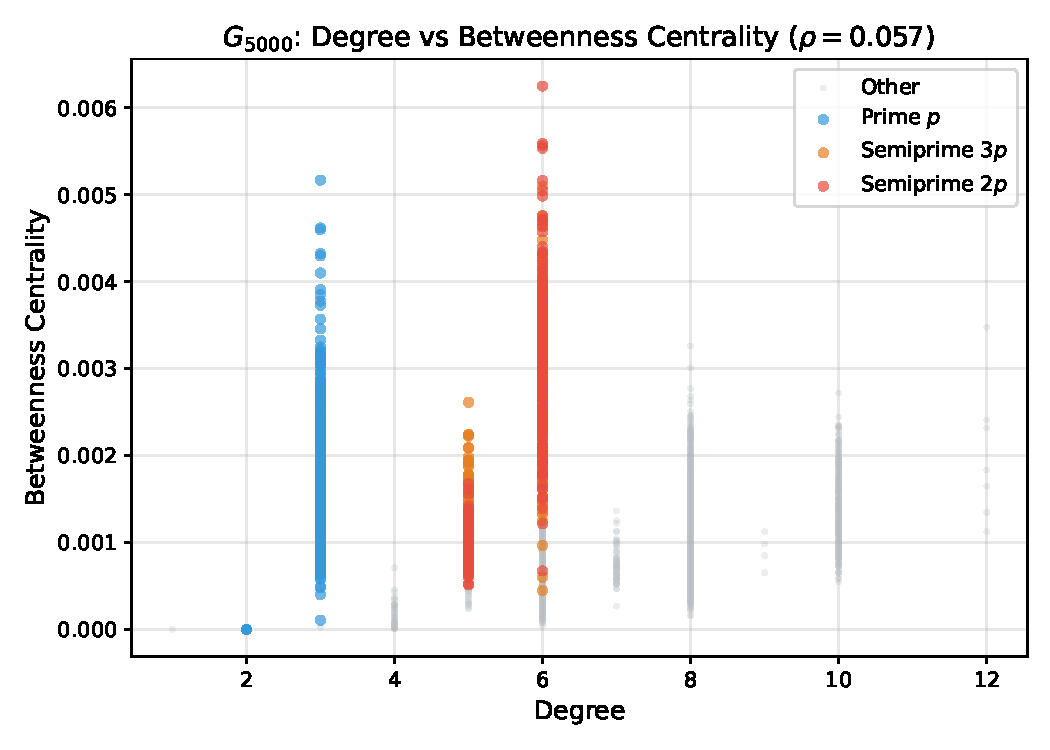
\includegraphics[width=0.85\textwidth]{fig_degree_vs_bc.pdf}
\caption{Degree versus betweenness centrality in $G_{5000}$.
Semiprimes $2p$ (red) and $3p$ (orange) cluster at degree~$6$ with high betweenness,
while primorials (grey, high degree) have moderate betweenness.
The correlation is $\rho = 0.057$.}
\label{fig:deg_vs_bc}

\noindent\textbf{Alt text:} Scatter plot showing degree on the x-axis (ranging from 2 to 12) versus betweenness centrality on the y-axis for all nodes in $G_{5000}$. Red dots representing semiprimes $2p$ and orange dots representing $3p$ are clustered at degree 6 with the highest betweenness values (up to 0.006). Grey dots at higher degrees (8--12) representing primorials show moderate betweenness values below 0.002. Blue dots representing bare primes appear at degree 3 with low betweenness.
\end{figure}

\subsection{Highway betweenness distribution}

\begin{table}[ht]
\centering
\caption{Distribution of betweenness among multiples of large primes ($N = 2000$).}\label{tab:highway}
\begin{tabular}{@{}rcccc@{}}
\toprule
$p$ & BC($p$) & BC($2p$) & BC($3p$) & $\text{BC}(2p) / \Sigma$ \\
\midrule
503 & 0.00391 & 0.00579 & 0.00389 & 42.6\% \\
509 & 0.00489 & 0.00686 & 0.00453 & 42.2\% \\
521 & 0.00302 & 0.00530 & 0.00361 & 44.5\% \\
541 & 0.00365 & 0.00522 & 0.00359 & 41.9\% \\
557 & 0.00486 & 0.00727 & 0.00477 & 43.0\% \\
\bottomrule
\end{tabular}
\end{table}

Node $2p$ consistently captures the largest share of betweenness among the highway nodes
of each large prime~$p$, with a mean share of $\approx 43\%$. Since $p$ (a bare prime)
has only degree~$3$, it receives less traffic despite being a highway endpoint. Node $3p$,
though it has degree~$6$ like $2p$, sits on the $3$-highway (sparser than the $2$-highway),
confirming the access-cost argument of Theorem~\ref{thm:bottleneck}.

\subsection{Routing cost U-shape}

\begin{table}[ht]
\centering
\caption{Average shortest-path distance from 500 random nodes to each multiple $kp$ ($N = 2000$).}\label{tab:ushape}
\begin{tabular}{@{}rccc@{}}
\toprule
$p$ & $\EE[d(\cdot, p)]$ & $\EE[d(\cdot, 2p)]$ & $\EE[d(\cdot, 3p)]$ \\
\midrule
503 & 5.96 & \textbf{5.69} & 5.96 \\
509 & 5.92 & \textbf{5.70} & 5.90 \\
521 & 5.93 & \textbf{5.68} & 5.99 \\
523 & 5.93 & \textbf{5.69} & 5.98 \\
541 & 5.99 & \textbf{5.85} & 6.17 \\
\bottomrule
\end{tabular}
\end{table}

For every tested prime, $2p$ has the lowest average distance from random sources,
confirming that it is the most globally accessible node on each highway
(Figure~\ref{fig:ushape}).

\begin{figure}[ht]
\centering
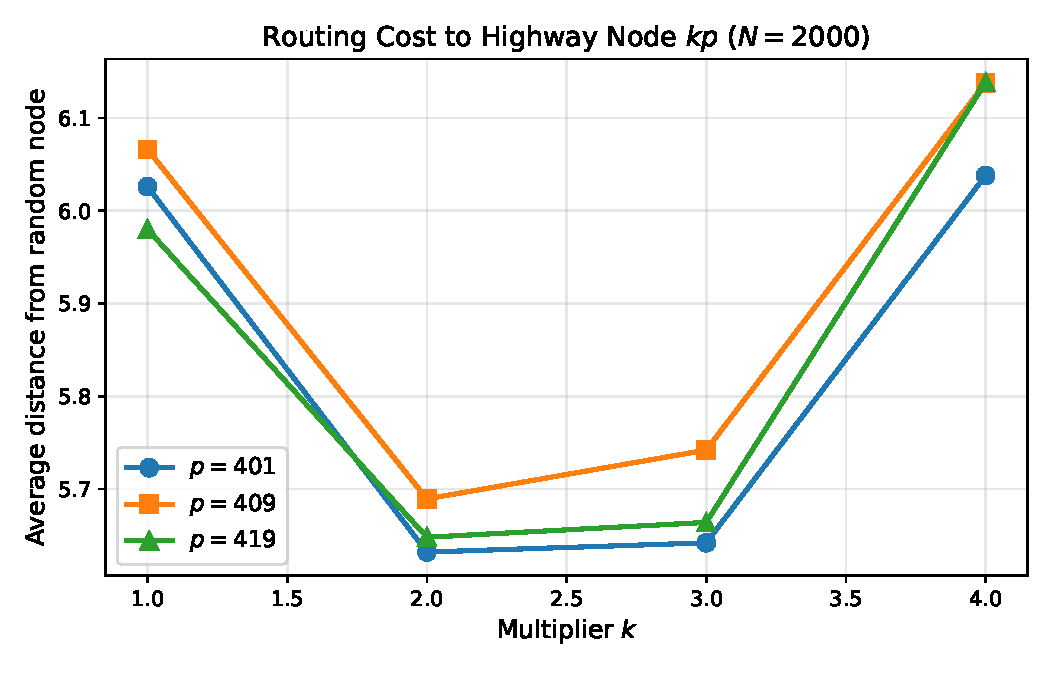
\includegraphics[width=0.75\textwidth]{fig_ushape.pdf}
\caption{Average shortest-path distance from $500$ random nodes to highway node $kp$,
for three primes $p$ in $G_{2000}$.
The minimum at $k = 2$ confirms that $2p$ is the most globally accessible on-ramp.}
\label{fig:ushape}

\noindent\textbf{Alt text:} Line plot with multiplier $k$ (1 to 4) on the x-axis and average shortest-path distance on the y-axis for three primes ($p = 401, 409, 419$). All three curves show a clear minimum at $k = 2$, with distances rising for $k = 1$ (bare prime) and $k \ge 3$, forming a U-shape that confirms node $2p$ is the most globally accessible.
\end{figure}


% ====================================================================
\section{Discussion}
% ====================================================================

Our findings reveal a structural paradox in arithmetic graphs.
The vertices that appear most important by degree are the primorials,
which have many distinct prime factors and sit on many highways;
yet they do not control the most shortest-path traffic.
The true bottlenecks are semiprime vertices where a dense local highway
(the $2$- or $3$-highway) crosses a sparse global one (a large-prime highway).

The phenomenon has a natural routing-theoretic explanation: a vertex's betweenness depends not on how many highways it serves, but on how \emph{essential} it is to each highway it serves.
A primorial sits on many highways but each highway has many possible stops. A semiprime $2p$ sits on only two highways, but on the $p$-highway there are at most three stops and $2p$ is the easiest to reach from a random source. 

\begin{conjecture}\label{conj:scaling}
As $N \to \infty$, the Pearson correlation $\rho(\deg, \BC)$ in $G_N$ converges to a non-positive limit;
in particular it changes sign at some finite $N_*$ and remains non-positive for all $N \ge N_*$.
Equivalently, for every $\varepsilon > 0$ there exists $N_0(\varepsilon)$ such that for all $N \ge N_0$,
the highest-betweenness vertex of $G_N$ is a semiprime of the form $2p$ or $3p$ with $p > N/4$.
\end{conjecture}

The seven exact-BC measurements in Table~\ref{tab:dominance} place the sign change in the interval
$N_* \in (10\,000,\, 20\,000)$, with $\rho$ continuing to drift downward at $N = 50\,000$.
The negative-limit version of Conjecture~\ref{conj:scaling} is the strongest reading of the data;
the weaker statement $\rho \to 0$ would also be a useful theorem, but seven scales alone cannot
adjudicate between the two limits. The reason to favour the negative-limit version is that, by
Corollary~\ref{cor:decorrelation}, the maximum-degree vertices have $\BC \to 0$ while
the maximum-BC vertices stay at degree~$6$. In the regime where these tails dominate the joint
distribution, $\Cov(\deg, \BC)$ becomes increasingly driven by the negative association between
high-$\omega$ primorials and small BC. A formal derivation that $\rho < 0$ in the limit
is left as an open problem.


\medskip
\noindent\textbf{Wider ramifications.}
The sparsity--accessibility trade-off is not unique to arithmetic graphs.
The same structural paradox can in principle arise in any network whose structure mixes dense local connections with sparse global ones:
a low-degree vertex that bridges a dense region to a sparse one can capture more betweenness than the high-degree hubs of the dense region.
This has practical implications for network resilience analysis, where standard methods focus on protecting high-degree hubs but the actual cut vertices may be the inconspicuous bridges identifiable only by betweenness.
Arithmetic graphs provide a deterministic, parameter-free model in which the phenomenon can be analyzed without recourse to random-graph assumptions. 

More speculatively, the fact that semiprimes $2p$ occupy a
structurally privileged position in the multiplicative landscape
of the integers may connect to computational number theory:
the routing geometry of $G_N$ encodes how addition and multiplication
interact, and understanding which integers act as bottlenecks
in this interaction could inform algorithmic approaches to
factorization and primality testing.


% ====================================================================
\section*{Data and code availability}
% ====================================================================

The Python scripts that build $G_N$, compute the exact betweenness centralities reported in Tables~\ref{tab:dominance}--\ref{tab:top10},
and produce all figures are available at
\url{https://github.com/tobiascanavesi/arithmetic-graph-primes}.
The repository includes the JSON output of the betweenness computations for $N \in \{500, 1000, 2000, 5000, 10\,000, 20\,000, 50\,000\}$,
so the tables and figures can be regenerated without re-running the multi-hour Brandes computation.

% ====================================================================
\section*{Use of generative AI}
% ====================================================================

The author used the generative AI tool Claude Opus~4.6 (Anthropic, 2025) for assistance with Python
code development for the betweenness-centrality computations and for \LaTeX\ formatting and copy-editing.
All mathematical content---including the definitions, theorems, proofs, conjectures, and the conceptual framework---is the original work of the author.
The author takes full responsibility for the accuracy and integrity of the manuscript.

\begin{thebibliography}{99}

\bibitem{Brandes2001}
Brandes U. A faster algorithm for betweenness centrality.
\emph{J Math Sociol} 2001;\textbf{25}:163--77.

\bibitem{ChandraDasgupta2005}
Chandra AK, Dasgupta S. A small world network of prime numbers.
\emph{Physica A} 2005;\textbf{357}(3--4):436--46.

\bibitem{ErdosSaias1995}
Erd\H{o}s P, Saias E. Sur le graphe divisoriel.
\emph{Acta Arith.} 1995;\textbf{73}(2):189--98.

\bibitem{ErdosSarkozy1997}
Erd\H{o}s P, S\'ark\"ozy GN. On cycles in the coprime graph of integers.
\emph{Electron. J. Combin.} 1997;\textbf{4}(2):R8.

\bibitem{Freeman1977}
Freeman LC. A set of measures of centrality based on betweenness.
\emph{Sociometry} 1977;\textbf{40}:35--41.

\bibitem{Hagberg2008}
Hagberg AA, Schult DA, Swart PJ. Exploring network structure, dynamics, and function using NetworkX.
In: \emph{Proceedings of the 7th Python in Science Conference (SciPy 2008)}, 11--15.

\bibitem{Hardy1979}
Hardy GH, Wright EM. \emph{An Introduction to the Theory of Numbers},
5th edn. Oxford: Oxford University Press, 1979.

\bibitem{KoukoulopoulosMaynard2020}
Koukoulopoulos D, Maynard J. On the Duffin--Schaeffer conjecture.
\emph{Ann. of Math.} 2020;\textbf{192}(1):251--307.

\bibitem{MelottiSaias2020}
Melotti P, Saias E. On path partitions of the divisor graph.
\emph{Acta Arith.} 2020;\textbf{192}(4):329--39.

\bibitem{Mertens1874}
Mertens F. Ein Beitrag zur analytischen Zahlentheorie.
\emph{J. Reine Angew. Math.} 1874;\textbf{78}:46--62.

\bibitem{NetworKit2016}
Staudt CL, Sazonovs A, Meyerhenke H. NetworKit: a tool suite for large-scale complex network analysis.
\emph{Network Science} 2016;\textbf{4}(4):508--30.

\bibitem{Pomerance2018}
Pomerance C. The first function and its iterates.
In: Butler S, Cooper J, Hurlbert G, eds., \emph{Connections in Discrete Mathematics: A Celebration of the Work of Ron Graham}.
Cambridge University Press; 2018, p. 125--38.

\bibitem{Pomerance1979}
Pomerance C. The prime number graph.
\emph{Math. Comp.} 1979;\textbf{33}(145):399--408.

\bibitem{Pomerance1983}
Pomerance C. On the longest simple path in the divisor graph.
\emph{Congressus Numerantium} 1983;\textbf{40}:291--304.

\bibitem{SanderSander2016}
Sander JW, Sander T. Recent developments on the edge between number theory and graph theory.
In: \emph{From Arithmetic to Zeta-Functions: Number Theory in Memory of Wolfgang Schwarz}.
Springer; 2016, p. 463--82.

\bibitem{SinghSantha2023}
Santhakumaran AP, Singh R. Brief survey on divisor graphs and divisor function graphs.
\emph{AKCE Int. J. Graphs Comb.} 2023;\textbf{20}(2):217--25, doi:10.1080/09728600.2023.2234979.

\bibitem{Watts1998}
Watts DJ, Strogatz SH. Collective dynamics of `small-world' networks.
\emph{Nature} 1998;\textbf{393}:440--2.

\end{thebibliography}

\end{document}
